%
%Не забыть:
%--------------------------------------
%Вставить колонтитулы, поменять название на титульнике



%--------------------------------------

\documentclass[a4paper, 12pt]{article} 

%--------------------------------------
%Russian-specific packages
%--------------------------------------
%\usepackage[warn]{mathtext}
\usepackage[T2A]{fontenc}
\usepackage[utf8]{inputenc}
\usepackage[english,russian]{babel}
\usepackage[intlimits]{amsmath}
\usepackage{esint}
%--------------------------------------
%Hyphenation rules
%--------------------------------------
\usepackage{hyphenat}
\hyphenation{ма-те-ма-ти-ка вос-ста-нав-ли-вать}
%--------------------------------------
%Packages
%--------------------------------------
\usepackage{amsmath}
\usepackage{amssymb}
\usepackage{amsfonts}
\usepackage{amsthm}
\usepackage{latexsym}
\usepackage{mathtools}
\usepackage{etoolbox}%Булевые операторы
\usepackage{extsizes}%Выставление произвольного шрифта в \documentclass
\usepackage{geometry}%Разметка листа
\usepackage{indentfirst}
\usepackage{wrapfig}%Создание обтекаемых текстом объектов
\usepackage{fancyhdr}%Создание колонтитулов
\usepackage{setspace}%Настройка интерлиньяжа
\usepackage{lastpage}%Вывод номера последней страницы в документе, \lastpage
\usepackage{soul}%Изменение параметров начертания
\usepackage{hyperref}%Две строчки с настройкой гиперссылок внутри получаеммого
\usepackage[usenames,dvipsnames,svgnames,table,rgb]{xcolor}% pdf-документа
\usepackage{multicol}%Позволяет писать текст в несколько колонок
\usepackage{cite}%Работа с библиографией
\usepackage{subfigure}% Человеческая вставка нескольких картинок
\usepackage{tikz}%Рисование рисунков
\usepackage{float}% Возможность ставить H в положениях картинки
% Для картинок Моти
\usepackage{misccorr}
\usepackage{lscape}
\usepackage{cmap}

\usepackage{mhchem}


\usepackage{graphicx,xcolor}
\graphicspath{{Pictures/}}
\DeclareGraphicsExtensions{.pdf,.png,.jpg}

%----------------------------------------
%Список окружений
%----------------------------------------
\newenvironment {theor}[2]
{\smallskip \par \textbf{#1.} \textit{#2}  \par $\blacktriangleleft$}
{\flushright{$\blacktriangleright$} \medskip \par} %лемма/теорема с доказательством
\newenvironment {proofn}
{\par $\blacktriangleleft$}
{$\blacktriangleright$ \par} %доказательство
%----------------------------------------
%Список команд
%----------------------------------------
\newcommand{\grad}
{\mathop{\mathrm{grad}}\nolimits\,} %градиент

\newcommand{\diver}
{\mathop{\mathrm{div}}\nolimits\,} %дивергенция

\newcommand{\rot}
{\ensuremath{\mathrm{rot}}\,}

\newcommand{\Def}[1]
{\underline{\textbf{#1}}} %определение

\newcommand{\RN}[1]
{\MakeUppercase{\romannumeral #1}} %римские цифры

\newcommand {\theornp}[2]
{\textbf{#1.} \textit{ #2} \par} %Написание леммы/теоремы без доказательства

\newcommand{\qrq}
{\ensuremath{\quad \Rightarrow \quad}} %Человеческий знак следствия

\newcommand{\qlrq}
{\ensuremath{\quad \Leftrightarrow \quad}} %Человеческий знак равносильности

\renewcommand{\phi}{\varphi} %Нормальный знак фи

\newcommand{\me}
{\ensuremath{\mathbb{E}}}

\newcommand{\md}
{\ensuremath{\mathbb{D}}}



%\renewcommand{\vec}{\overline}




%----------------------------------------
%Разметка листа
%----------------------------------------
\geometry{top = 3cm}
\geometry{bottom = 2cm}
\geometry{left = 1.5cm}
\geometry{right = 1.5cm}
%----------------------------------------
%Колонтитулы
%----------------------------------------
\pagestyle{fancy}%Создание колонтитулов
\fancyhead{}
%\fancyfoot{}
%\fancyhead[R]{\textsc{Получение и измерение вакуума}}%Вставить колонтитул сюда
%----------------------------------------
%Интерлиньяж (расстояния между строчками)
%----------------------------------------
%\onehalfspacing -- интерлиньяж 1.5
%\doublespacing -- интерлиньяж 2
%----------------------------------------
%Настройка гиперссылок
%----------------------------------------
\hypersetup{				% Гиперссылки
	unicode=true,           % русские буквы в раздела PDF
	pdftitle={Заголовок},   % Заголовок
	pdfauthor={Автор},      % Автор
	pdfsubject={Тема},      % Тема
	pdfcreator={Создатель}, % Создатель
	pdfproducer={Производитель}, % Производитель
	pdfkeywords={keyword1} {key2} {key3}, % Ключевые слова
	colorlinks=true,       	% false: ссылки в рамках; true: цветные ссылки
	linkcolor=blue,          % внутренние ссылки
	citecolor=blue,        % на библиографию
	filecolor=magenta,      % на файлы
	urlcolor=cyan           % на URL
}
%----------------------------------------
%Работа с библиографией (как бич)
%----------------------------------------
\renewcommand{\refname}{Список литературы}%Изменение названия списка литературы для article
%\renewcommand{\bibname}{Список литературы}%Изменение названия списка литературы для book и report
%----------------------------------------
\begin{document}
	\begin{titlepage}
		\begin{center}
			$$$$
			$$$$
			$$$$
			$$$$
			% To be reworked
			{\Large{НАЦИОНАЛЬНЫЙ ИССЛЕДОВАТЕЛЬСКИЙ УНИВЕРСИТЕТ}}\\
			\vspace{0.1cm}
			{\Large{ВЫСШАЯ ШКОЛА ЭКОНОМИКИ}}\\
			\vspace{0.25cm}
			{\large{Факультет физики}}\\
			\vspace{4cm}
			{\Huge\textbf{{Лабораторная работа}}}\\%Общее название
			\vspace{1cm}
			{\LARGE{<<Рентгеновская дифрактометрия>>}}\\%Точное название
			\vspace{2cm}
			{Работу выполнил студент 3 курса}\\
			{Захаров Сергей Дмитриевич}
			\vfill
			
\includegraphics[width=0.2\linewidth]{HSElogo}
			\vfill
			Москва\\
			2020
		\end{center}
	\end{titlepage}

Для анализа были предоставлены данные, представленные на рисунке \ref{fig:data}. Вместе ними нам дается знание, что они были получены на излучении \ce{CuK-\alpha 1}, а в веществе должны присутствовать \ce{O}, \ce{La}, \ce{Sr}, \ce{Mn}.

\begin{figure}[H]
	\centering
	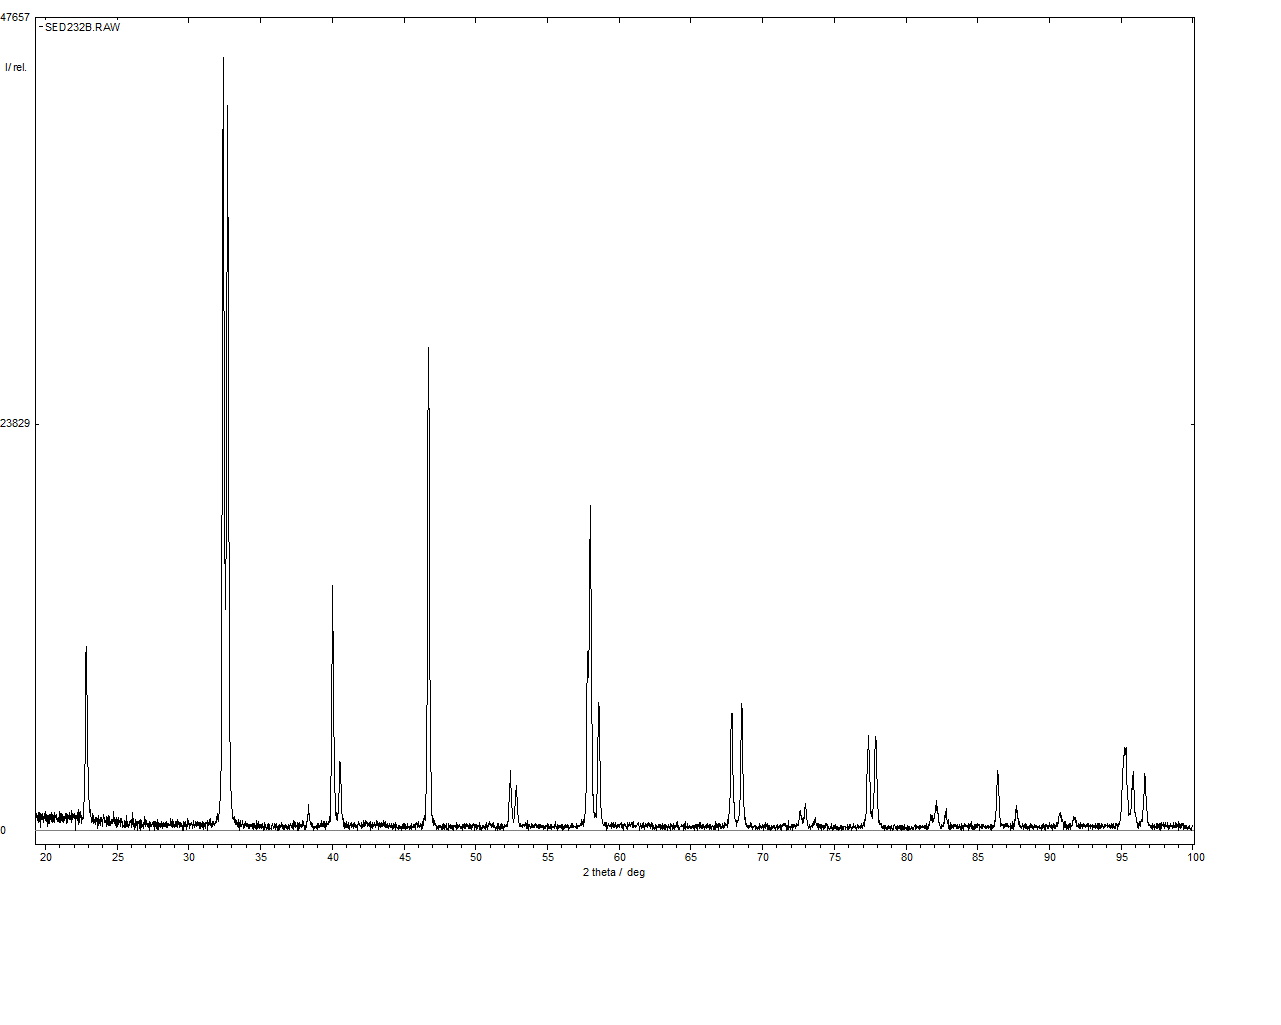
\includegraphics[width=\linewidth]{data}
	\caption{Предоставленные для анализа данные}
	\label{fig:data}
\end{figure}

На основании этого, с помощью программы Match! и встроенной в нее базы данных попытаемся найти в последней что-то, похожее на имеющиеся у нас данные. Для этого сперва исключим все записи, не имеющие указанных элементов, после чего последовательно начнем просматривать оставшиеся.

В результате некоторого поиска было обнаружено, что наилучшее совпадение (даже без подгонки) обеспечивает формула \ce{La_{0.67} Sr_{0.33} Mn O_3} (запись 96-153-3313). Промежуточные данные представлены на рисунке \ref{fig:theor_no_podg}.

\begin{figure}[H]
	\centering
	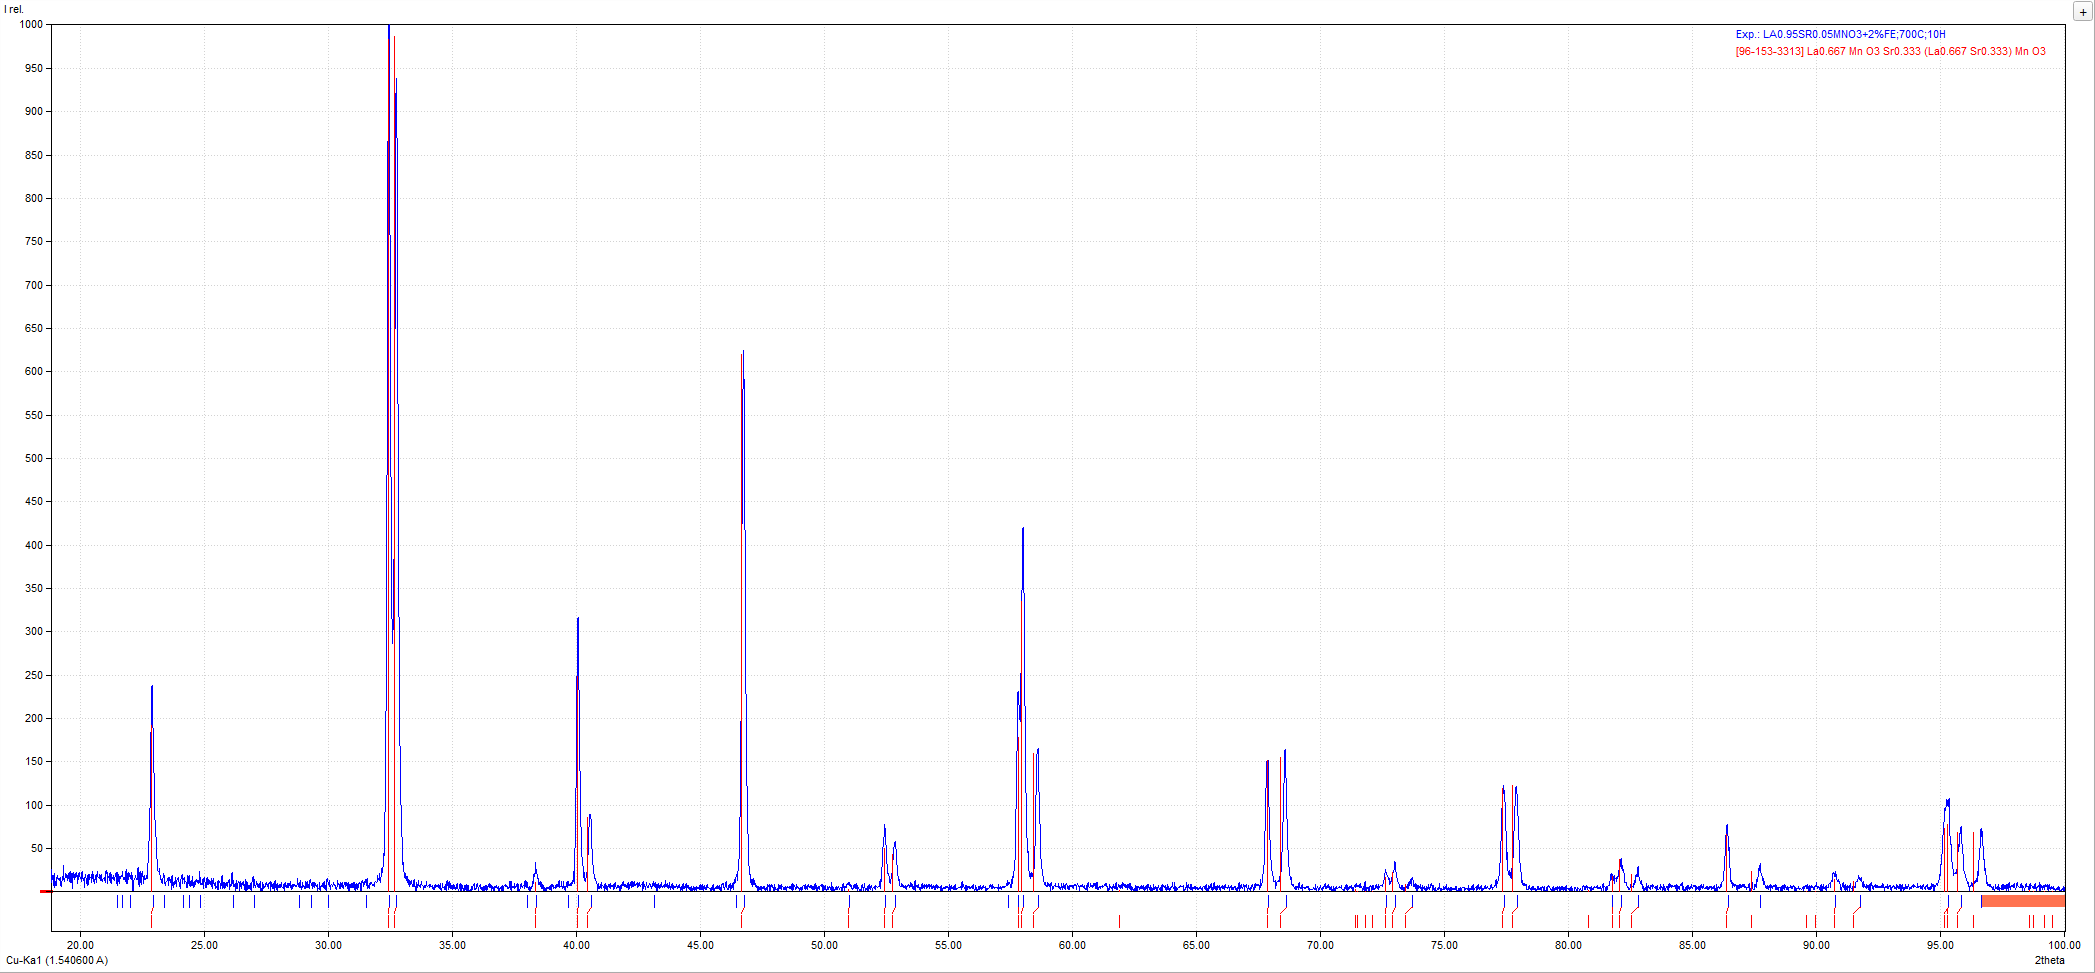
\includegraphics[width=\linewidth]{Theor_no_podg}
	\caption{Результат поиска совпадений в программе Match!}
	\label{fig:theor_no_podg}
\end{figure}

Теперь, зная из карточки из записи необходимые параметры (а именно формулу, параметры решетки и положение атомов), а также тип излучения, мы можем с помощью программы PowderCell фитануть полученные графики. По результатам была получена картина, представленная на рисунке \ref{fig:PDC}. Сравнительно небольшие $R$ ($R_p = 20.38, R_{wp} =50.61, R_{exp} = 0.68$) свидетельствуют о том, что процесс фита в целом прошел успешно, что в очередной раз подтверждает правильность выбранной нами формулы \ce{La_{0.67} Sr_{0.33} Mn O_3}. 

\begin{figure}[H]
	\centering
	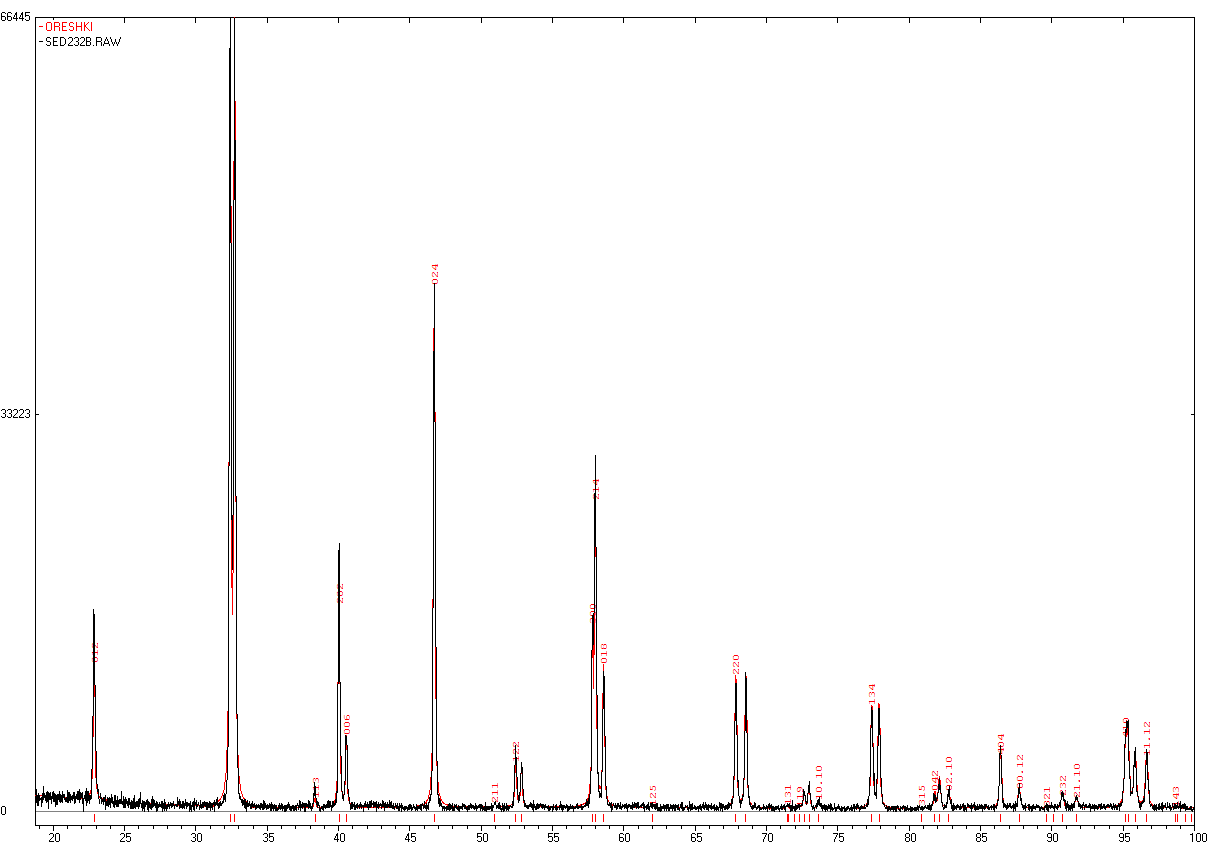
\includegraphics[width=\linewidth]{Theor}
	\caption{Данные после прохода через PowderCell}
	\label{fig:PDC}
\end{figure}


\newpage


\begin{thebibliography}{1}
	\bibitem{Practicum}
	Рентгендифракционные методы изучения структуры монокристаллов, поликристаллических и аморфных материалов
\end{thebibliography}




\end{document}